\subsection{Randomised timing}


Randomised timing of message sent by $j$ at time $t_j$ and received by $i$. Let,
\begin{align}
	\chi_{i,j} = t_j+\tau_{i,j}+\chi(w),
\end{align}
be the randomised time of receipt of arrival time of message from $j$ by $i$.

We require $T_0\geq\tau_\mathrm{max}$ such that all honest nodes are acknowledged under worst-case latency.

Considering the two limiting cases are $\tau_{i,j}=0$ and $\tau_{i,j}=\tau_\mathrm{max}$, we have,
\begin{align}
	\chi_{i,j}^{(\mathrm{min})} &= \chi(w) + t_j,\nonumber\\
	\chi_{i,j}^{(\mathrm{max})} &= \chi(w) + t_j + \tau_\mathrm{max}.
\end{align}

The respective likelihoods of acceptance are,
\begin{align}
	\mathbb{P}(\chi_{i,j}^{(\mathrm{min})} \leq T_0),\nonumber\\
	\mathbb{P}(\chi_{i,j}^{(\mathrm{max})} \leq T_0).
\end{align}


\begin{align}
	\mathbb{P}(\chi_{i,j} \leq T_0) = \begin{cases}
		0, &\chi_{i,j}<0\\
		\frac{\chi_{i,j}}{w}, &0\leq \chi_{i,j}\leq w\\
		1, &\chi_{i,j}>w
	\end{cases},
\end{align}
where the random variable has PDF,
\begin{align}
	f_{\chi(w)}(t) = \begin{cases}
		\frac{1}{w}, &0\leq t\leq w\\
		0, &\mathrm{otherwise}
	\end{cases},
\end{align}
with CDF
\begin{align}
	F_{\chi(w)}(t) = \begin{cases}
		0, &t<0\\
		\frac{t}{w}, &0\leq t\leq w\\
		1, &t>w
	\end{cases}.
\end{align}
The term \mbox{$\tau_{i,j}/w$} is the uncertainty associated with lack of knowledge of $\tau_{i,j}$, which may be treated as a random variable. When \mbox{$\mathrm{Var}(\tau_{i,j})\ll w$} this is vanishing. Thus for \mbox{$w\gg \mathrm{Var}(\tau_{i,j})$} the randomisation masks the latency profile.

\subsection{Miscellaneous notes}

Upon post-selection the accepted set of participants are in unanimous agreement on set membership.
Attestations for accepted participants.

Although PoCs execute in synchronous environments they are asynchronous objects.

Nodes evaluate time-compliance based on time-of-receipt, enforcing an effective lower-bound on delta. All time-of-receipts (sender excluded) are commit-revealed. Consensus-time at each synchronous step of the protocol is with respect to the time-of-receipts of messages associated with the respective protocol stage: acceptance, consensus and compliance.

Dynamic networks: Dynamic network membership: network algorithmically implements policies on network’s nodes and parameters. Could be democratic.

Proof-of-work artificially ties monetary dynamics with its gross inefficiency, where transaction cost …

Nodes' time accuracy is economically self-incentivised towards accuracy.

Deferred proof-of-consensus: provide only proof of random subsets but not consensus, which can be made at a later point.

Node announcements are:
1. Bid.
2. Consensus on participants (assigns random subsets).
3. Consensus on transaction.
4. Consensus on compliance.

Eliminate timestamping service. Instead maintain local lists of message arrival times.

Eq 5.7: add lexographical ordering when hashing bids together into global key.

Commit-reveal ensures announcements are made blindly, independent of those made by other nodes, preventing race-time conditions arising whereby dishonest nodes inform their own announcements based on those of others.

Nodes operate their own priority queues for incoming consensus requests. In a floating market these could be prioritised by their offered transaction fee. The transaction fee is received exclusively by the delegate node presenting the bid to the network. Within the network all nodes contribute the same work to performing consensus as they receive. Nodes are incentivised to present the most profitable PoCs to the network, while transaction initiators are incentivised to present bids to the cheapest nodes. Under efficient market assumptions this drives the network towards uniform transaction fees.

r can be interpreted as the maximum tolerable dissent to maintain epsilon-security, above which the PoC is invalid as it defies the signing network’s policies.

Statements can refer to arbitrary external sources or sign PoCs provisioned by other networks.

Purpose of expanding networks is diversification, which reduces r, enabling smaller consensus sets given epsilon.

Transaction hierarchies: consensus can be delegated to lower cost side networks or different network types, such as roaming networks, which only execute transactions between themselves. From primary ledger transfer credits to fully-back the risk exposure of the side-network’s consensus policy.
Would be less against compromise with higher r.

Nodes adopt retreat strategies in accordance with trust hierarchies.

Multiple nodes under common ownership correlates their individual $r_i$. Increases consensus bandwidth.

Markowitz theory for reducing r.

How does payout work? Non-compliant nodes burn the fee?

Minimising r is incentivised via reduced consensus set size. Consider correlated risk of joining two networks. When is it best to join? If the two r’s are perfectly positively correlated (i.e the same) the overall r is just r. If the two are negatively correlated? Consider Markowitz theory for risk diversification theory.

Any majority of signatures from the consensus set on the final compliance vote constitutes a proof-of-consensus. As majorities are not unique neither are proofs-of-consensus, but are all equivalent proofs of the same consensus.

$O(n)$ execution time for n nodes, network energy consumption scales as $O(n^2)$.

From an arbitrary pool of consensus-signed statements a blockchain is a directed linear graph of chronologically ordered statements, defined by the function deciding which subset of statements form the chain. The blockchain function

$f_B({statements},time) -> {chain_statements}$

$f_B({s},t_0) \subseteq f_B({s},t_1) for t_1>t_0$
(set is non-decreasing, non-repudiation)

As blockchains must retain retrospective integrity, here $\{s\}$ denotes the statement pool for all time.

This property implies the blockchain function can be expressed inductively as deciding which statement (n+1) follows the previous one (n).

As it is possible for multiple satisfying blocks to follow a given block this can conversely be expressed as an elimination function which prunes a tree graph to a linear one. Choosing the earliest satisfying block as the block addition rule is the only rule guaranteeing that requirement [2] is upheld.

Conversely this can be considered an elimination procedure,

Zero-epsilon network allocates the entire network as consensus set.

Think about queue allocation

Defence against majority takeover:
From the perspective of an honest player, who knows they are honest themselves, allying with nodes that vote in common provides a strategic group defence to retreat-and-fork defence.

* Map trust tree to network partition structure, define relationships when $r_i$ is node-dependent.

r cannot be quantified. Map r to tolerated threshold ratio of dissent. Define as threshold for retreat-and-fork (network partition). As r represents the ratio of adversaries for which epsilon-security is defined, it therefore represents a publicly-known trigger at which retreat-and-fork is necessary to maintain epsilon-security, now defined relative to a subnet. Adopting this strategy enforces epsilon-security in consensus integrity from the perspective of nodes within a given alliance. From an external perspective, blind to all conspiracies, trusting the majority alliance is optimal.

Not time-stamping messages of non-compliant nodes is not considered non-compliance. Are only required at the final consensus.

Quantum randomness: while w and x are independently uniformly distributed, collectively they are not as they are correlated via the TCF instance.

epsilon is the security parameter of the network.

w and x certifiably random, secured by the TCF.

https://arxiv.org/pdf/1804.00640.pdf

https://quantum-journal.org/papers/q-2022-09-19-807/

https://arxiv.org/pdf/2112.05156.pdf

On majority vote by median: No minority act can undermine the compliance of others (the majority).

The integer steps in the synchronous protocol are defined relative to a date constant modulo their periodicity.

Consensus on transaction bundles obeys an algorithmic constant of the associated blockchain.

Consensus is formed on statements, arbitrary decision problems  $f_s(\cdot)\to \{0,1\}$ whose complexity is bounded by the network's nodes. Could be classical or quantum, BPP or BQP, subject to practical constraints.

Use for outsourced computation. Consensus notarises the validity of the output. If bidder is unable to verify the computation themselves and must have assurance of the integrity of outcomes, consensus notarises integrity of outcome.

Inefficiency due to replication. With N=1 there is no duplication of computation although the executing node remains randomly assigned. In this trivial case we have epsilon=r security.

A protocol acts on a subset of consensus proofs. A blockchain is a protocol that acts on PoCs associated with transactions on a specific chain.

There is no need for a blockchain to ensure the integrity of the current state of the ledger. Instead PoCs act notarise only the current state of the ledger. No need for hash-list to ensure integrity. Transaction history is not required to ensure integrity of current state, which is inherently epsilon-secure, independent of transaction history. A PoC-signed state register is intrinsically epsilon-secure.

epsilon is dependent on the trigger r at which strategic retreat is enforced.

Distributed computation: Allocate different algorithms to different consensus nodes. So long as they can form consensus of combined outcomes.

Mutating state register following an arbitrary update rule executed by the signing consensus nodes, an arbitrary distributed computation.

PoC signs the validity of arbitrary decision problems, for which one application is smart contracts.

A blockchain is a subset of PoCs post-selected on packets satisfying the blockchain rules, defining a chronologically ordered, directed linear graph.

Abolishing the notion of distinct, independent blockchains. Rather mutating state register

Cross-ledger transactions requires only that both recognise PoCs executing them.

No inherent notion of competing coins across different chains. Blockchains are implemented purely based on mutual recognition of the blockchain algorithm.

Sequence of subset reassignments by re-hashing local keys. These can all be calculated at once. We re-hash $N_c$ times allocating each node to form consensus on $N_c$ independent statements. Nodes via their participation contribute the same work as a full consensus, matching their bid requesting one, making it contribution neutral for all nodes.

The network's net computational and communications resources scale as $O(n^2)$ with small constants from a practical perspective. Communications: broadcast announcements; Computational: $O(n^2)$ in the number of hashes and $O(n)$ in the number of evaluations of the function defining question.

A valid PoC comprises:
* Any majority of nodes from a consensus set individually sign:
* Which consensus nodes were compliant and their announced consensus outcomes (proof of execution).
* Accepted bids and participant list signed by all participating network nodes (proof of random subsets).

Valid PoC is required to release deposit escrow.

Open networks: single consensus set acts as source of truth.
Open-bidding

On evolving ledgers:
PoCs can be retrospectively ignored if above a certain age.
A policy of not recognising PoCs above a certain age

Quantum case: deposit > cost of quantum computation.

Proof-of-storage has been raised as an alternative. Distributed algorithms based on proof of any kind of resource consumption is inherently wasteful if consumption scales super-linearly with network size. For consensus . Must be
Consensus algorithm must optimise algorithmic efficiency.

Inter-network atomic operations

An international racket driven by the greed of algorithmic inefficiency whose mobsters' opulent lifestyle...

Pseudo-randomness of hash functions.
Strong pre-image resistance.

Although it is super exponential it behaves itself: num bit-strings vs num permutations.

\section{Topology}

There are two distinct topologies, the evolution of networks and the evolution of which ones ledgers recognise.
Ledger’s evolve as a function of network topology.
Their intersection is a point of consideration.

A ledger may be a function of PoCs contributed by different consensus pools. At the protocol level a ledger is defined by arbitrary subsets of PoCs satisfying its rules.

\section{Structure of consensus space}

Elements of the powerset of S who cardinality is $\kappa\geq majority$.

Full consensus: where all nodes bid one transaction and participate in $N_C$ PoCs. Equality in the receipt of and contribution towards consensus. Allocation requires $N_C$ independent random partitions.

Space of network nodes maps to multiset of consensus space with multiplicity $N_C$ on all elements. Multiset maps back to set of network nodes.

\section{Consensus hierarchies}

%\begin{figure}
%	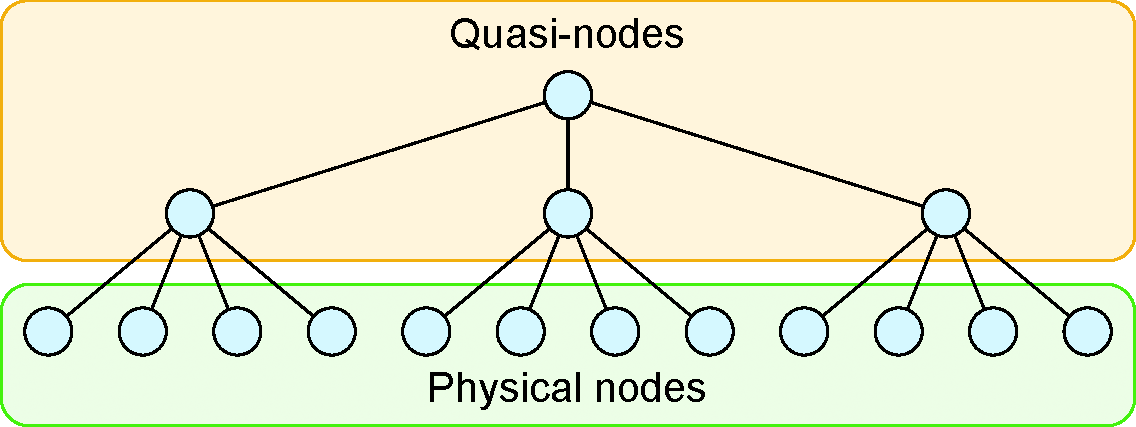
\includegraphics[width=\columnwidth]{figures/trust_hierarchy.pdf}
%	\caption{} \label{fig:trust_hierarchy}
%\end{figure}
